
\chapter{Background}
\section{Backgammon Rules}
To create a backgammon system, the rules and terminology must first be defined.
Backgammon is played by two opponents on a board consisting of 24 triangles called points. 
The points alternate in colour and are grouped into four quadrants of six points each.
These quadrants are the player's home board and outer board, and the opponent's home board and outer board. 
A region down the centre of the board, called the bar, separates the home and outer boards.

\begin{figure}[H]
    \centering
    
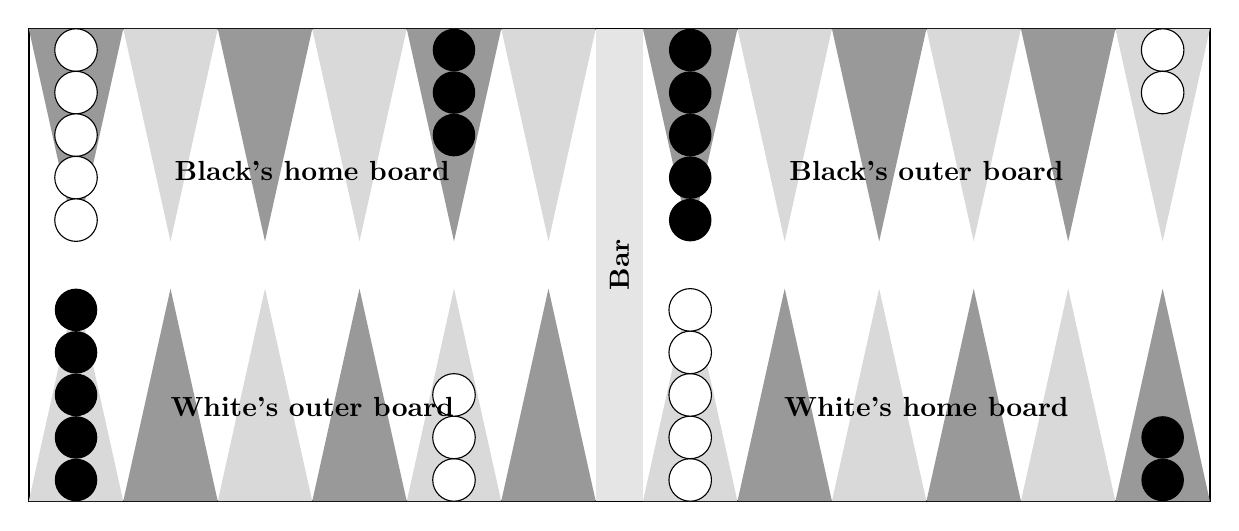
\begin{tikzpicture}[scale=0.3]
  % checker radius (in unscaled units)
  \def\r{0.9}

  % overall board
  \draw[thick] (0,0) rectangle (50,20);

  % the bar
  \fill[gray!20] (24,0) rectangle (26,20);
  \node[rotate=90] at (25,10) {\bfseries Bar};

  % bottom row of triangles (player side) — left half
  \foreach \i in {0,...,5} {
    \pgfmathsetmacro\x{4*\i}
    \fill[\ifodd\i gray!80\else gray!30\fi]
      (\x,0) -- (\x+4,0) -- (\x+2,9) -- cycle;
  }
  % bottom row of triangles (player side) — right half
  \foreach \i in {0,...,5} {
    \pgfmathsetmacro\x{26 + 4*\i}
    \fill[\ifodd\i gray!80\else gray!30\fi]
      (\x,0) -- (\x+4,0) -- (\x+2,9) -- cycle;
  }

  % top row of triangles (opponent side) — left half
  \foreach \i in {0,...,5} {
    \pgfmathsetmacro\x{4*\i}
    \fill[\ifodd\i gray!30\else gray!80\fi]
      (\x,20) -- (\x+4,20) -- (\x+2,11) -- cycle;
  }
  % top row of triangles (opponent side) — right half
  \foreach \i in {0,...,5} {
    \pgfmathsetmacro\x{26 + 4*\i}
    \fill[\ifodd\i gray!30\else gray!80\fi]
      (\x,20) -- (\x+4,20) -- (\x+2,11) -- cycle;
  }

  % --- starting checkers ---

  % Player (bottom) — white
  % 2 on 24-point → top, x-mid=48
  \pgfmathsetmacro\x{48}
  \foreach \j in {0,1} {
    \pgfmathsetmacro\y{20 - \r - \j*2*\r}
    \fill[white, draw=black] (\x,\y) circle (\r);
  }
  % 5 on 13-point → top, x-mid=2
  \pgfmathsetmacro\x{2}
  \foreach \j in {0,...,4} {
    \pgfmathsetmacro\y{20 - \r - \j*2*\r}
    \fill[white, draw=black] (\x,\y) circle (\r);
  }
  % 3 on 8-point  → bottom, x-mid=18
  \pgfmathsetmacro\x{18}
  \foreach \j in {0,...,2} {
    \pgfmathsetmacro\y{\r + \j*2*\r}
    \fill[white,draw=black] (\x,\y) circle (\r);
  }
  % 5 on 6-point  → bottom, x-mid=28
  \pgfmathsetmacro\x{28}
  \foreach \j in {0,...,4} {
    \pgfmathsetmacro\y{\r + \j*2*\r}
    \fill[white,draw=black] (\x,\y) circle (\r);
  }

  % Opponent (top) — black
  % 2 on 24-point → bottom, x-mid=2
  \pgfmathsetmacro\x{2}
  \foreach \j in {0,...,4} {    \pgfmathsetmacro\y{\r + \j*2*\r}
    \fill[black] (\x,\y) circle (\r);
  }
  % 5 on 13-point → bottom, x-mid=48
  \pgfmathsetmacro\x{48}
  \foreach \j in {0,1} {
    \pgfmathsetmacro\y{\r + \j*2*\r}
    \fill[black] (\x,\y) circle (\r);
  }
  % 3 on 8-point  → top, x-mid=32
  \pgfmathsetmacro\x{18}
  \foreach \j in {0,...,2} {
    \pgfmathsetmacro\y{20 - \r - \j*2*\r}
    \fill[black] (\x,\y) circle (\r);
  }
  % 5 on 6-point  → top, x-mid=22
  \pgfmathsetmacro\x{28}
  \foreach \j in {0,...,4} {
    \pgfmathsetmacro\y{20 - \r - \j*2*\r}
    \fill[black] (\x,\y) circle (\r);
  }

  % quadrant labels
  \node at (12,4)  {\bfseries White's outer board};
  \node at (38,4)  {\bfseries White's home board};
  \node at (12,14) {\bfseries Black's home board};
  \node at (38,14) {\bfseries Black's outer board};
  
  
  \end{tikzpicture}
    \caption{Backgammon board and starting positions of checkers}
    \label{fig:backgammonboard}
\end{figure}


% Setup
Each player begins with 15 checkers, which are placed on the board in a specific starting position, as shown in figure \ref{fig:backgammonboard}.
Checkers move in opposite directions towards their respective home boards (in figure \ref{fig:backgammonboard}, white moves anticlockwise and black moves clockwise).

% Objective
The objective of the game is for a player to move all 15 of their checkers into their home board and then bear them off (remove them from the board). 
The first player to bear off all their checkers wins the game.

% Starting the game
\subsection{Movement}
To start the game, each player rolls a die. 
The player with the higher number goes first and uses the numbers rolled by both players for their initial move. 
If they roll the same number, they roll again until different numbers appear.

% Turns
Players then alternate turns, rolling two dice at the beginning of each turn.

% Using the dice
A player must move their checkers according to the numbers shown on the dice. 
The two dice rolls represent two separate moves. 
For example, a roll of 5 and 3 (written as 5-3) means the player can move one checker 5 points and another checker 3 points, or move a single checker a total of 8 points (by moving it 5 points to an intermediate point, then 3 points further, or vice-versa), provided one of the intermediate landing points is not blocked by the opponent.

% Doubles
If a player rolls doubles (the same number on both dice), they can move four times the number shown on the dice. 
For example, a roll of 5-5 allows the player four moves of 5 points each (written as 5-5-5-5).

% Valid moves
A checker may only land on an open point, one not occupied by two or more opposing checkers. 
Points occupied by zero or one opposing checker are open. Any number of checkers of the same colour can occupy a single point.

If a player has legal moves available according to the dice roll, they must make them. 
If only one of the dice numbers allows a legal move, that move must be made. 
If either die allows a legal move but not both, the higher number must be played if possible. 
If neither die allows a legal move, the player forfeits their turn. 
If doubles are rolled and not all four moves can be made, the player must make as many moves as possible.

% Hitting
\subsection{Hitting and Re-entering}
If a checker lands on a point occupied by exactly one opposing checker (a blot), the opposing checker is hit and placed on the bar.
A player with one or more checkers on the bar cannot make any other moves until all their checkers on the bar have re-entered the game. 
A checker re-enters on the point in the opponent's home board corresponding to the number rolled on a die, provided that point is open. 
For example, if White has a checker on the bar and rolls a 3-5, they can re-enter on Black's 3-point if it is open, or on Black's 5-point if it is open. 
If neither corresponding point is open, the player forfeits their turn.

\subsection{Bearing off}
A player can only begin bearing off checkers once all 15 of their checkers are within their own home board.

A checker can be borne off a point if the number rolled on a die matches the point number (e.g., rolling a 4 allows bearing off a checker from the 4-point).
If a die roll is higher than the highest point on which the player has a checker, they may bear off a checker from the highest occupied point. 
For example, if a player rolls a 5 but has no checkers on the 5-point, but does have checkers on the 4-point, they can use the 6 to bear off a checker from the 4-point.

If a player can make a legal move using a die roll within their home board instead of bearing off, they are allowed to do so. However, if a checker can be borne off legally using a die roll, the player cannot choose to move a checker on a lower point if there are no checkers on points higher than the die roll. (The dice must be used to their highest possible value if possible, prioritising bearing off or moving from the highest points).

If a player's checker is hit while they are bearing off, they must re-enter that checker onto the bar and bring it back to their home board before they can resume bearing off.
\label{sec:rules}

\subsection{Backgammon Terminology}
TODO: not sure if i need this or should add to it
\begin{definition}[Blot]
A single exposed checker. Blots are disadvantageous as they can be hit.
\end{definition}

\begin{definition}[Hitting]
    The act of landing on a point occupied by a single opponent checker, sending the opponent's checker to the bar.
\end{definition}

\begin{definition}[Primes]
    A series of consecutive points that a player controls (with multiple pieces). Primes are effective at preventing an opponent from moving past.
\end{definition}

\begin{definition}[Anchors]
    A point in the opponent's home board occupied by two or more of the player's checkers.    
\end{definition}

\section{Existing Work}
\section{Game Design}
\section{AI and Games}

The development of AI for stochastic games has followed a separate path compared to deterministic games, due to major differences in the algorithms required. 
While traditional approaches for games like chess relied heavily on minimax search with alpha-beta pruning \cite{deepblue}, these techniques are less effective in games with chance elements due to the much larger branching factor when considering all possible dice rolls \cite{RussellNorvig}.

Early approaches to backgammon AI relied on evaluation functions created by backgammon experts and had limited depth lookahead \cite{berliner1980}. A significant breakthrough came with TD-Gammon, developed by Gerald Tesauro at IBM TODO, which used temporal difference learning (TD-$\lambda$) with a neural network to develop an evaluation function. TD-Gammon demonstrated that neural networks trained through self-play could learn complex decision making equal to world champions, without being explicitly programmed with backgammon specific strategies (Tesauro, 2002). TD-Gammon's success encouraged research in reinforcement learning and helped establish the application of neural network approaches for complex games (Sutton \& Barto, 2018).
